%%%%%%%%%%%%%%%%%%%%%%%%%%%%%%%%%%%%%%%%%%%%%%%%%%%
% PRESENTATION FOR TOM HEATON'S VISIT (11-07-2018)
% 
% Prithvi Thakur
% Geophysics research group
% Department of Earth and Environmental Science
% University of Michigan, Ann Arbor
%%%%%%%%%%%%%%%%%%%%%%%%%%%%%%%%%%%%%%%%%%%%%%%%%%%

\documentclass{beamer}

\mode<presentation> {
\usetheme{AnnArbor}
}

\usepackage{graphicx} % Allows including images
\usepackage{booktabs} % Allows the use of \toprule, \midrule and \bottomrule in tables
%\usepackage[export]{adjustbox} % To change the default alignment of image
\usepackage{subcaption} % Add subfigures to place figures side by side
\usepackage[absolute,overlay]{textpos}
%------------------------------------------------
%           TITLE PAGE INFORMATION
%------------------------------------------------
\title[EQ Cycles with DFZ]{Earthquake Cycle Simulations on a 2D Strike-Slip Fault Surrounded by Damaged Zones} 
\author{Prithvi Thakur}
\institute[UofM]
{
\medskip
University of Michigan \\ % Your institution for the title page
\medskip
\textit{prith@umich.edu} % Your email address
}
\date{01-10-2019} % Date, can be changed to a custom date
%------------------------------------------------

%%%%%%%%%%%%%%%%
\begin{document}

% TITLE PAGE
\begin{frame}
    \titlepage 
\end{frame}

% TABLE OF CONTENTS
\begin{frame}
    \frametitle{Overview}
    \begin{itemize}
        \item 2D Numerical simulation of long-term fault slip using a spectral element method. Fully dynamic scheme for nucleation, rupture propagation, and postseismic deformation integrated with the aseismic phase. 
        \item Strike-slip fault with mode III rupture (e.g., San Andreas), surrounded by a narrow damaged zone of low rigidity (Damaged Fault Zone).
        \item Spatial extent and material properties of damaged fault zones: how do they influence the earthquake sequence behavior?
    \end{itemize}
\end{frame}

% Research questions
\section{Research Questions}
\begin{frame}
    \frametitle{Research Questions}
    \begin{itemize}
        \item How does the damaged fault zone control the nucleation site (hypocenter) of the earthquakes? How does this change over subsequent cycles?
        \item What contributes to the power law behavior of earthquakes: is it the friction, or the material heterogeneities, or both?
        \item What other earthquake complexities can be explained by the damaged fault zone properties?
    \end{itemize}
\end{frame}

% MODEL DESCRIPTION
\section{Model Description}
\begin{frame}
    \frametitle{Model Description}
    \begin{figure}
        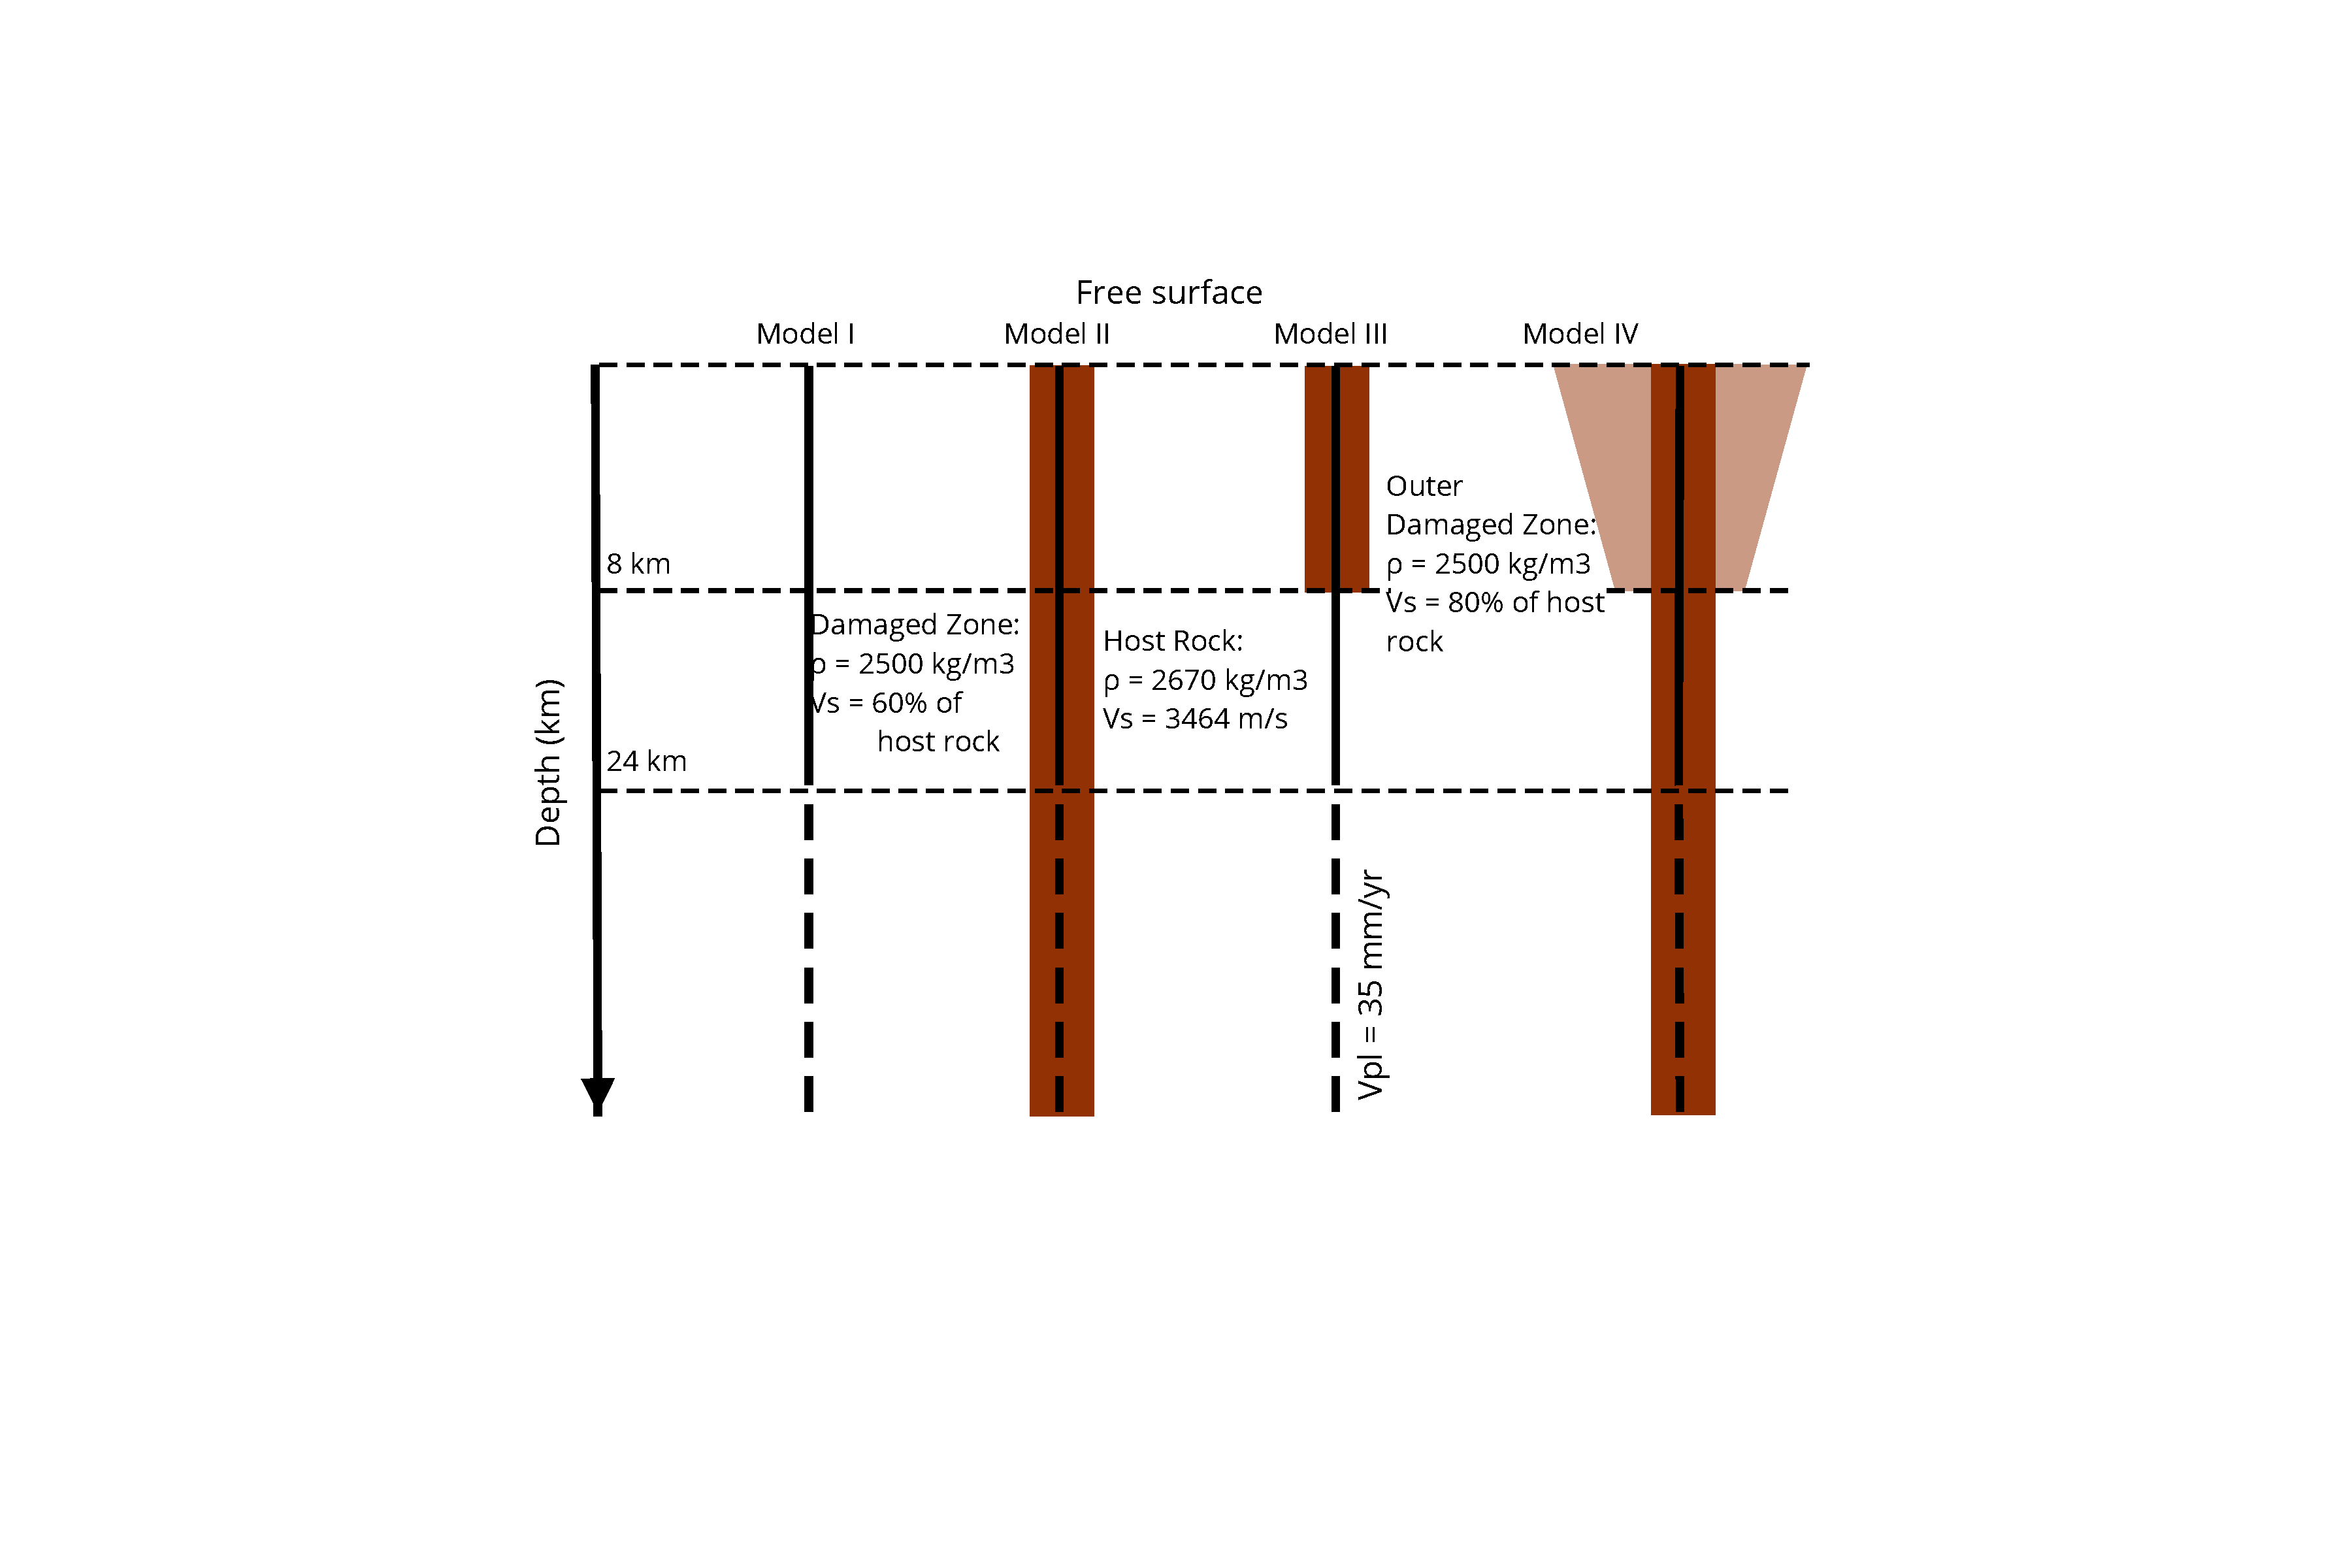
\includegraphics[width=1\linewidth]{images/fig2}
    \end{figure}
\end{frame}

% RESULTS PLOT
\section{Simulated Results}
\begin{frame}
    \frametitle{Simulated Results: Homogeneous Medium}
    \begin{figure}
        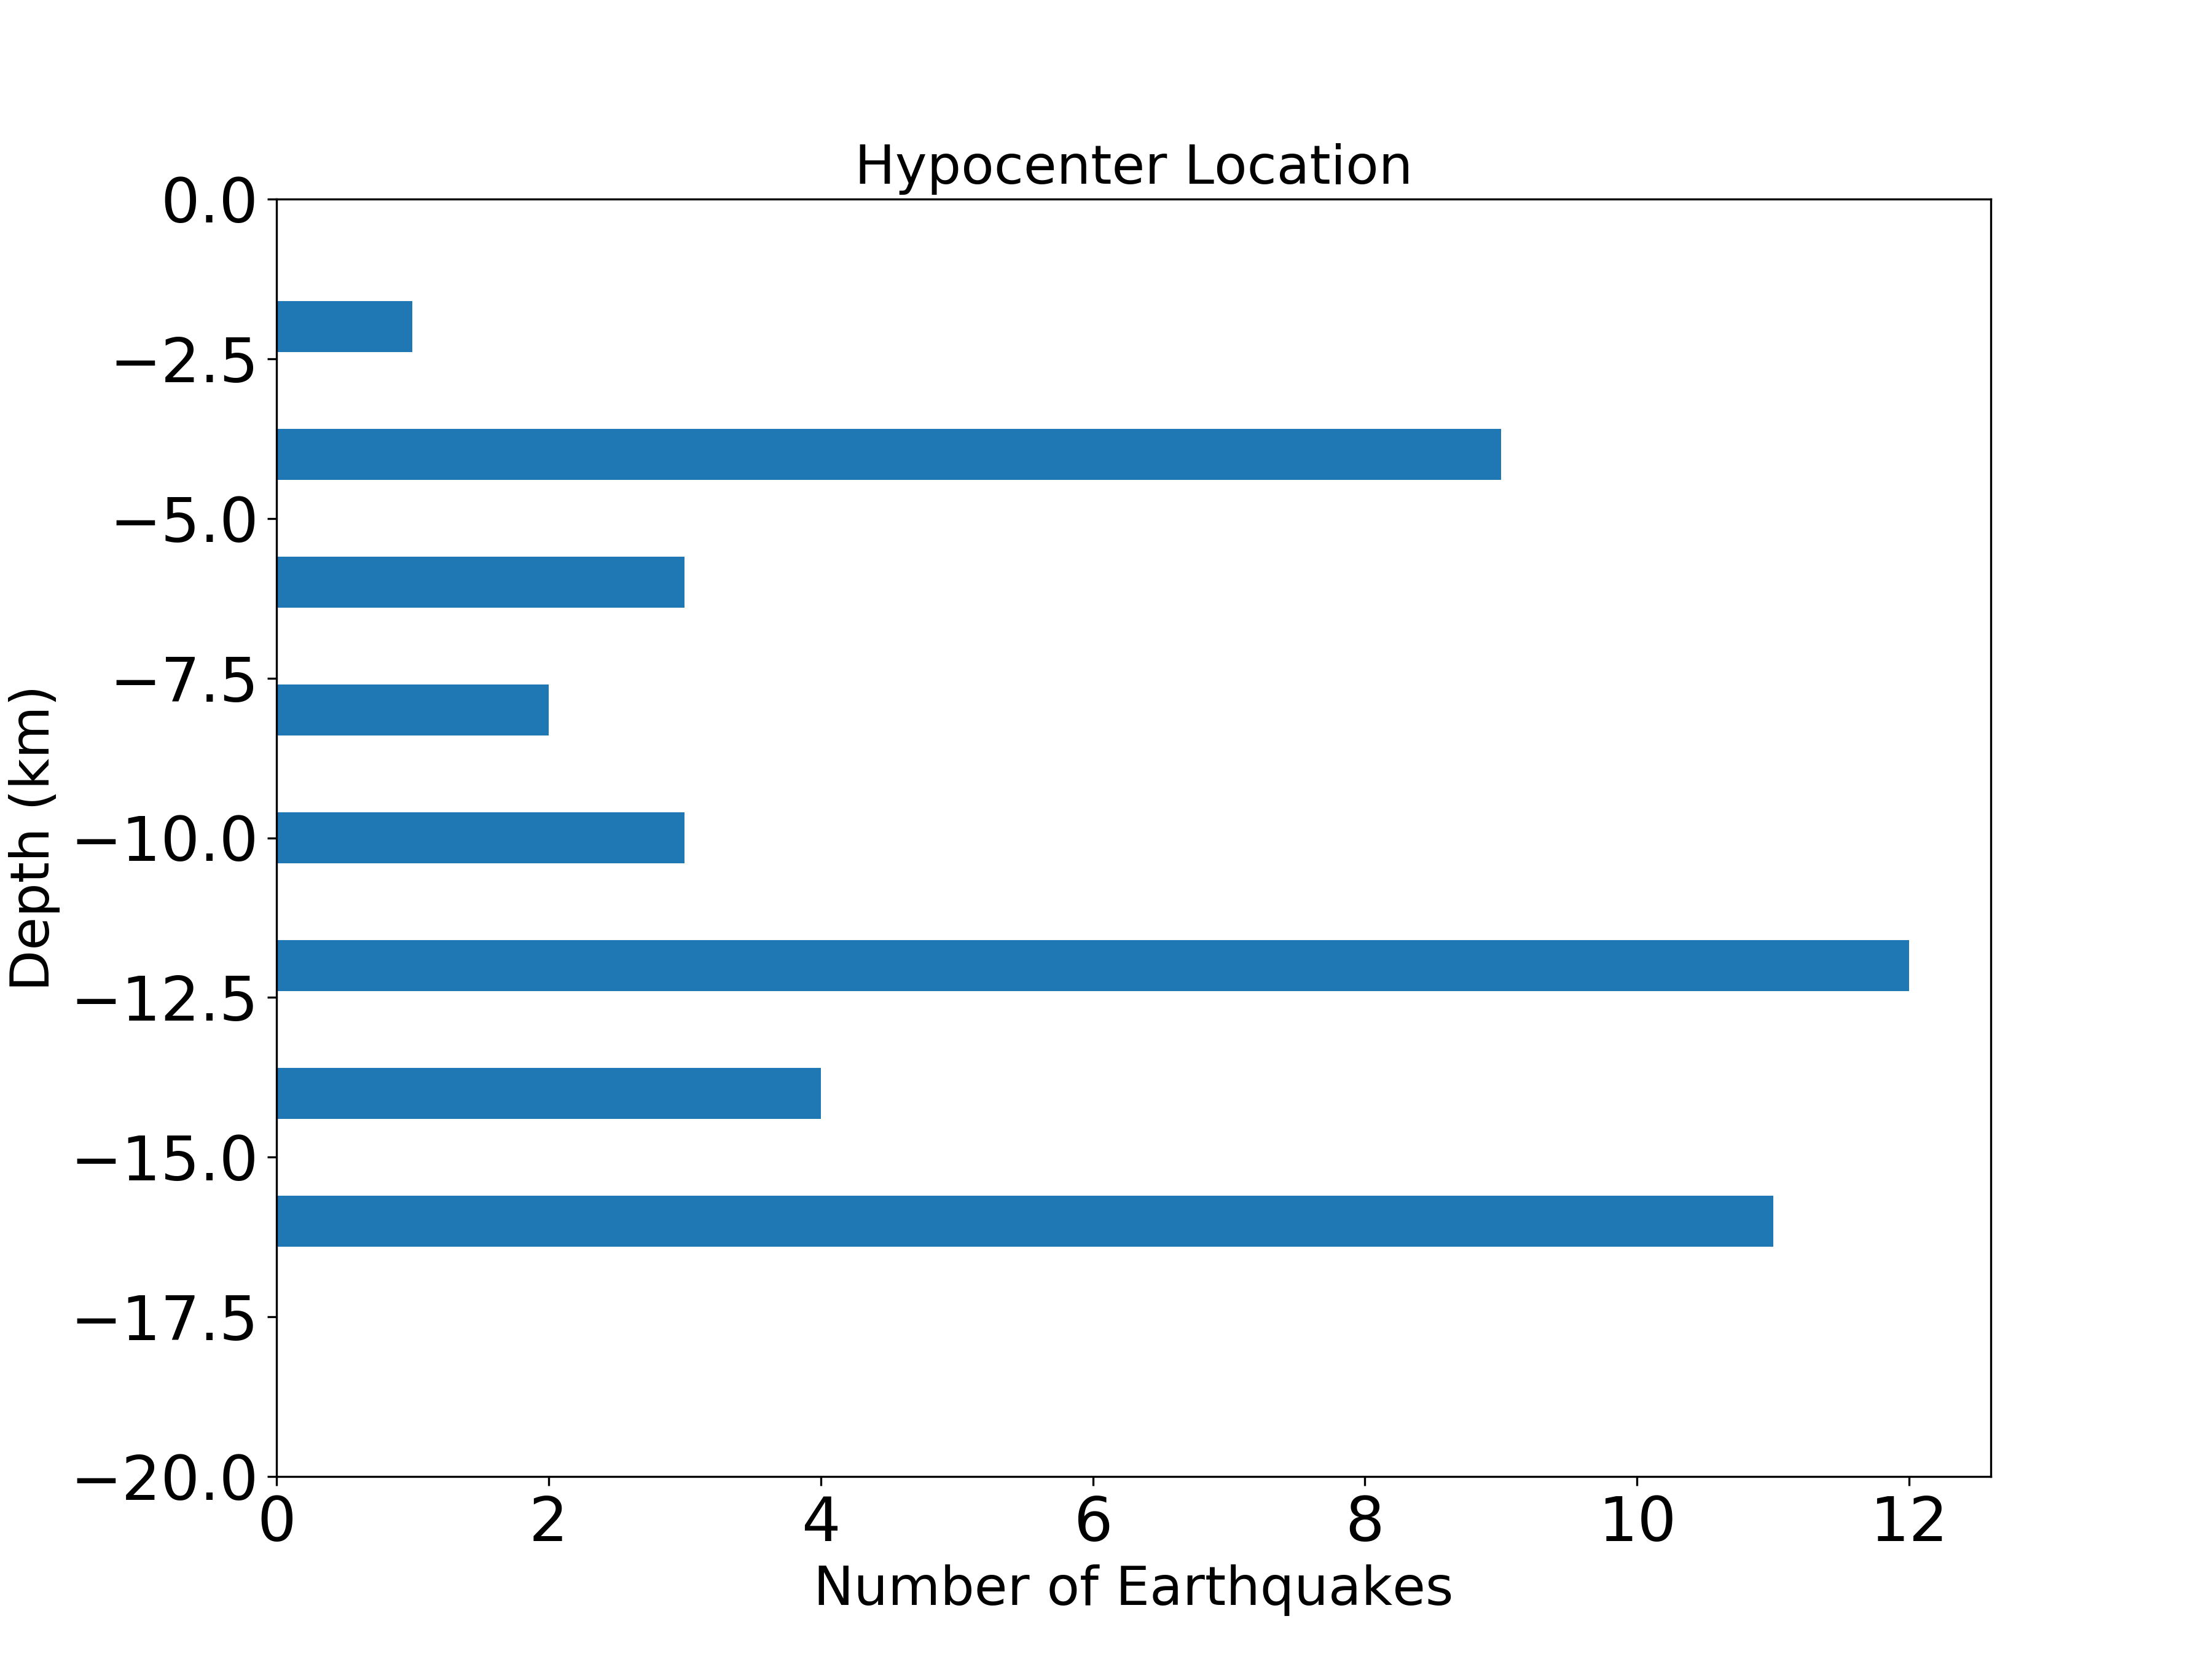
\includegraphics[width=0.5\linewidth]{images/homodc4.png} 
        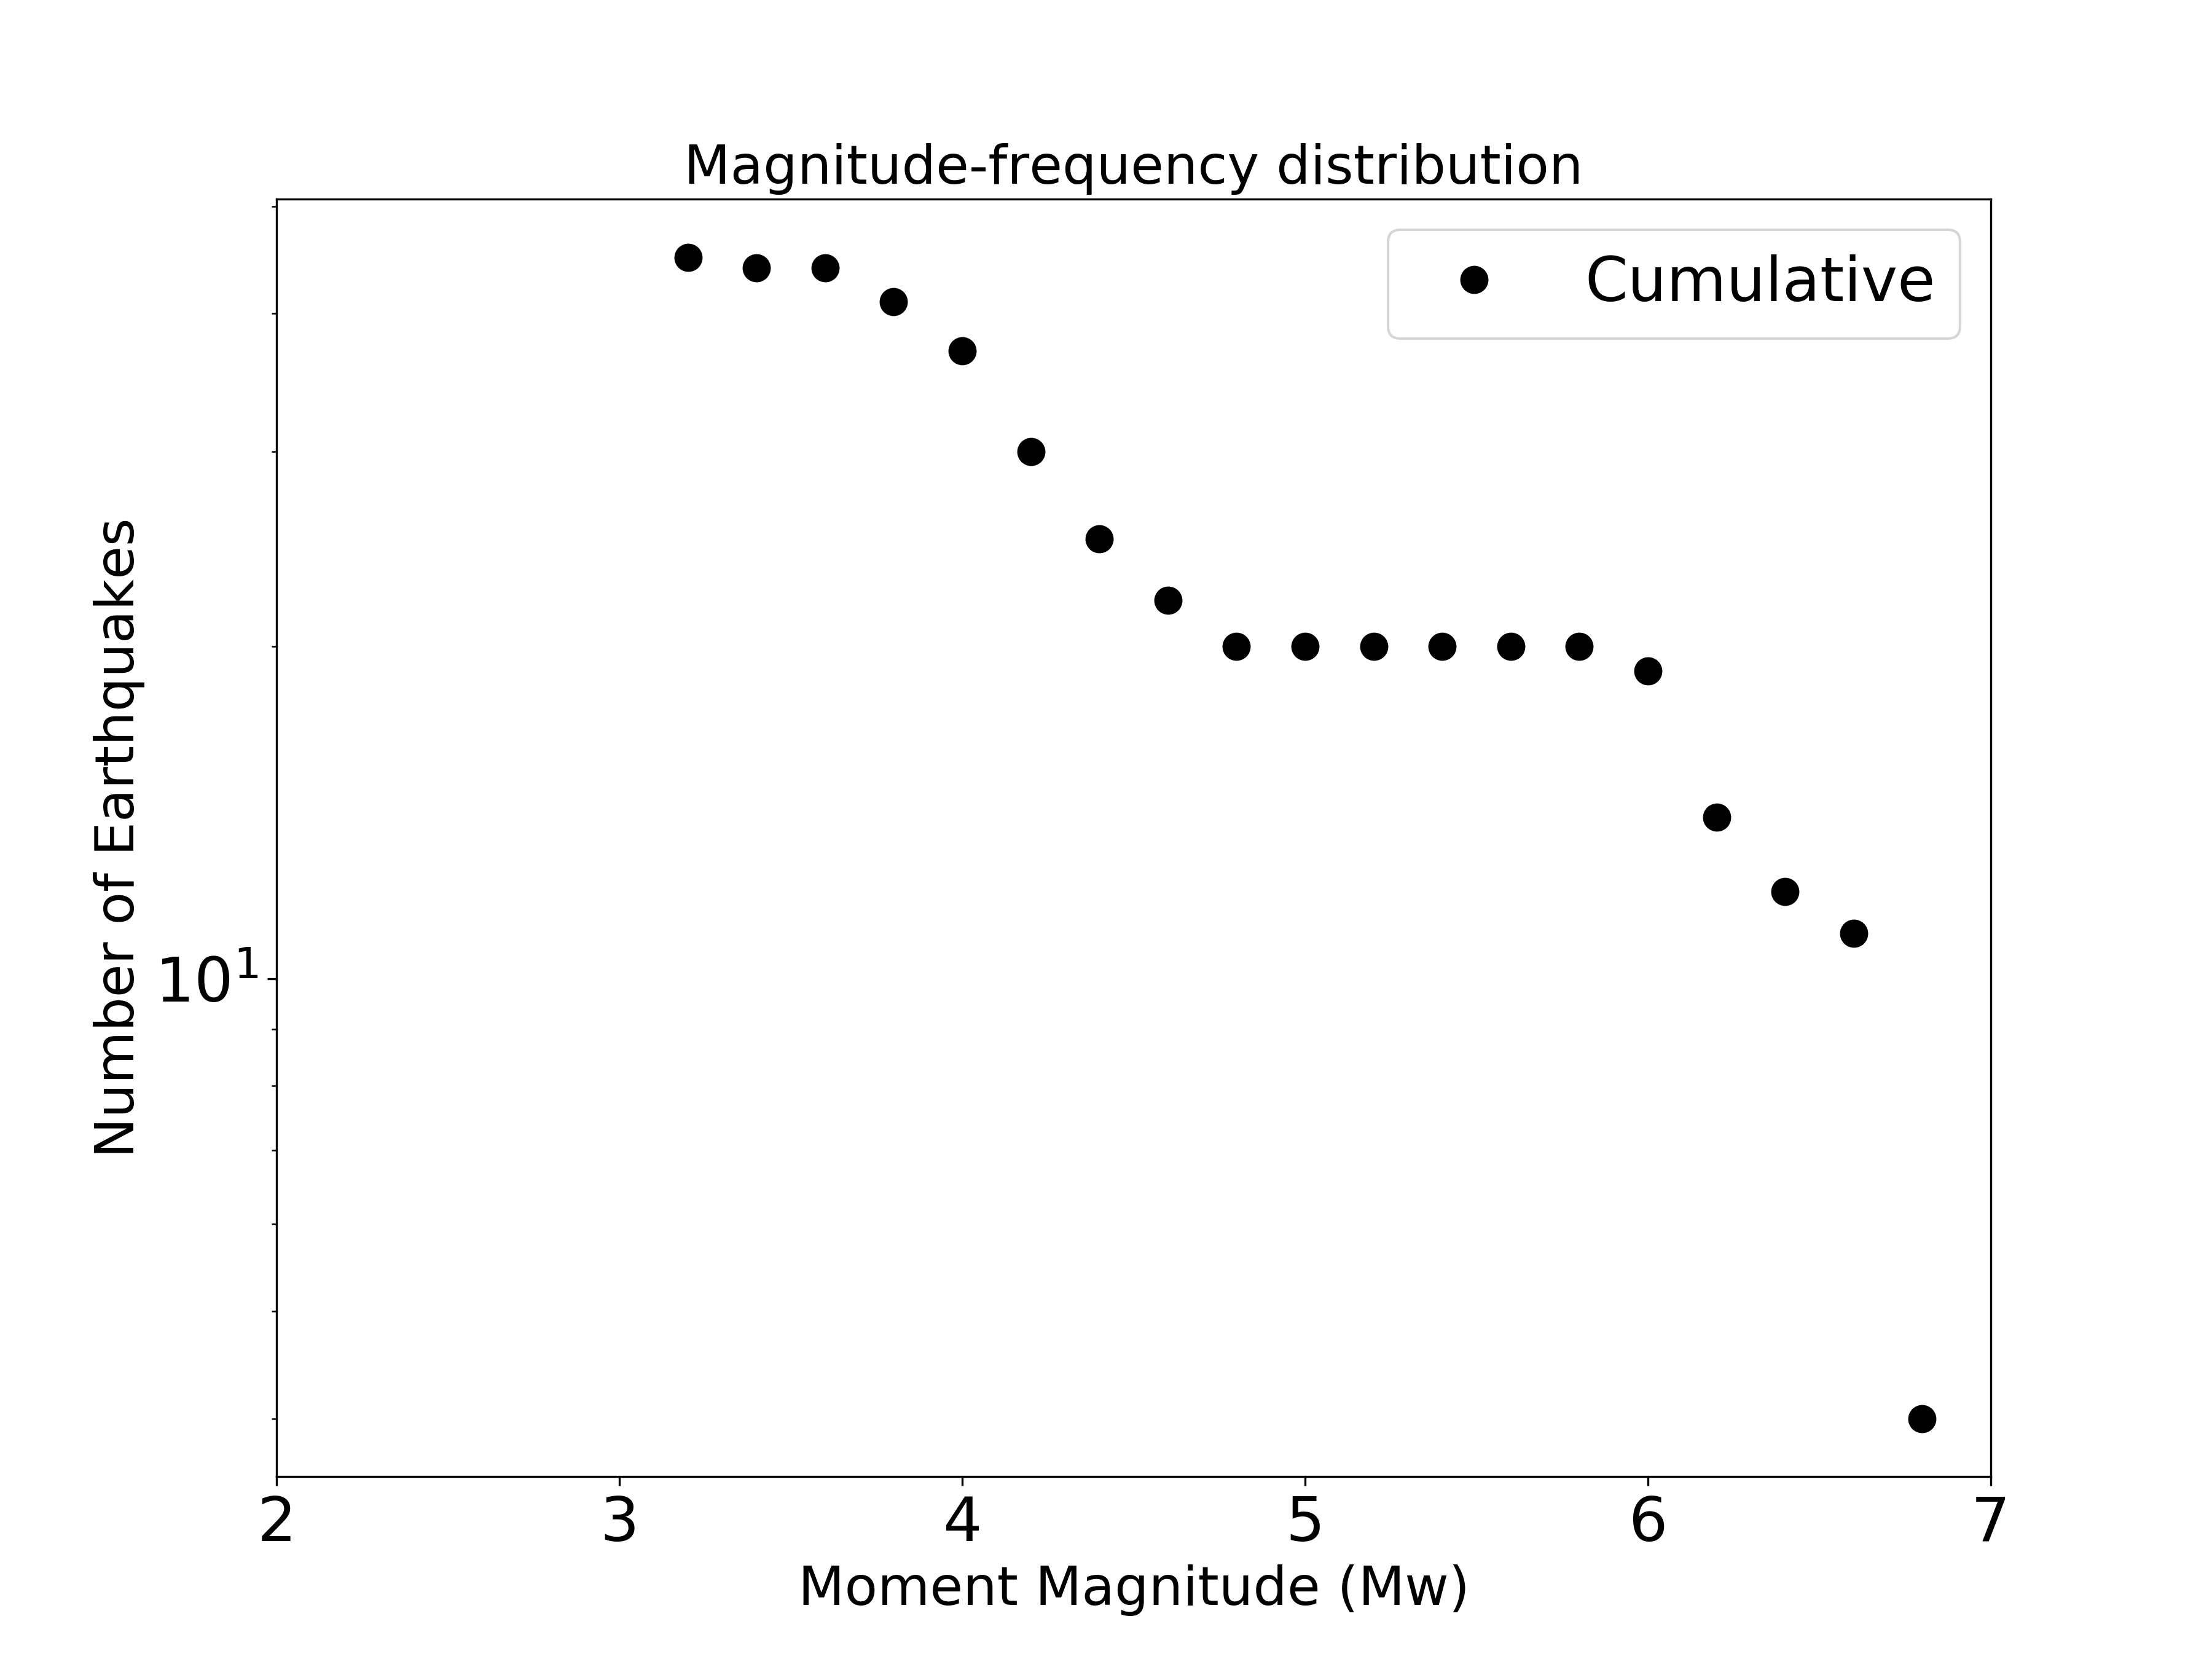
\includegraphics[width=0.5\linewidth]{images/homodc4_mfd.png} 
    \end{figure}
\end{frame}

\begin{frame}
    \frametitle{Simulated Results: Fault Zone throughout the domain }
    \begin{figure}
        \begin{subfigure}[b]{0.5\textwidth}
            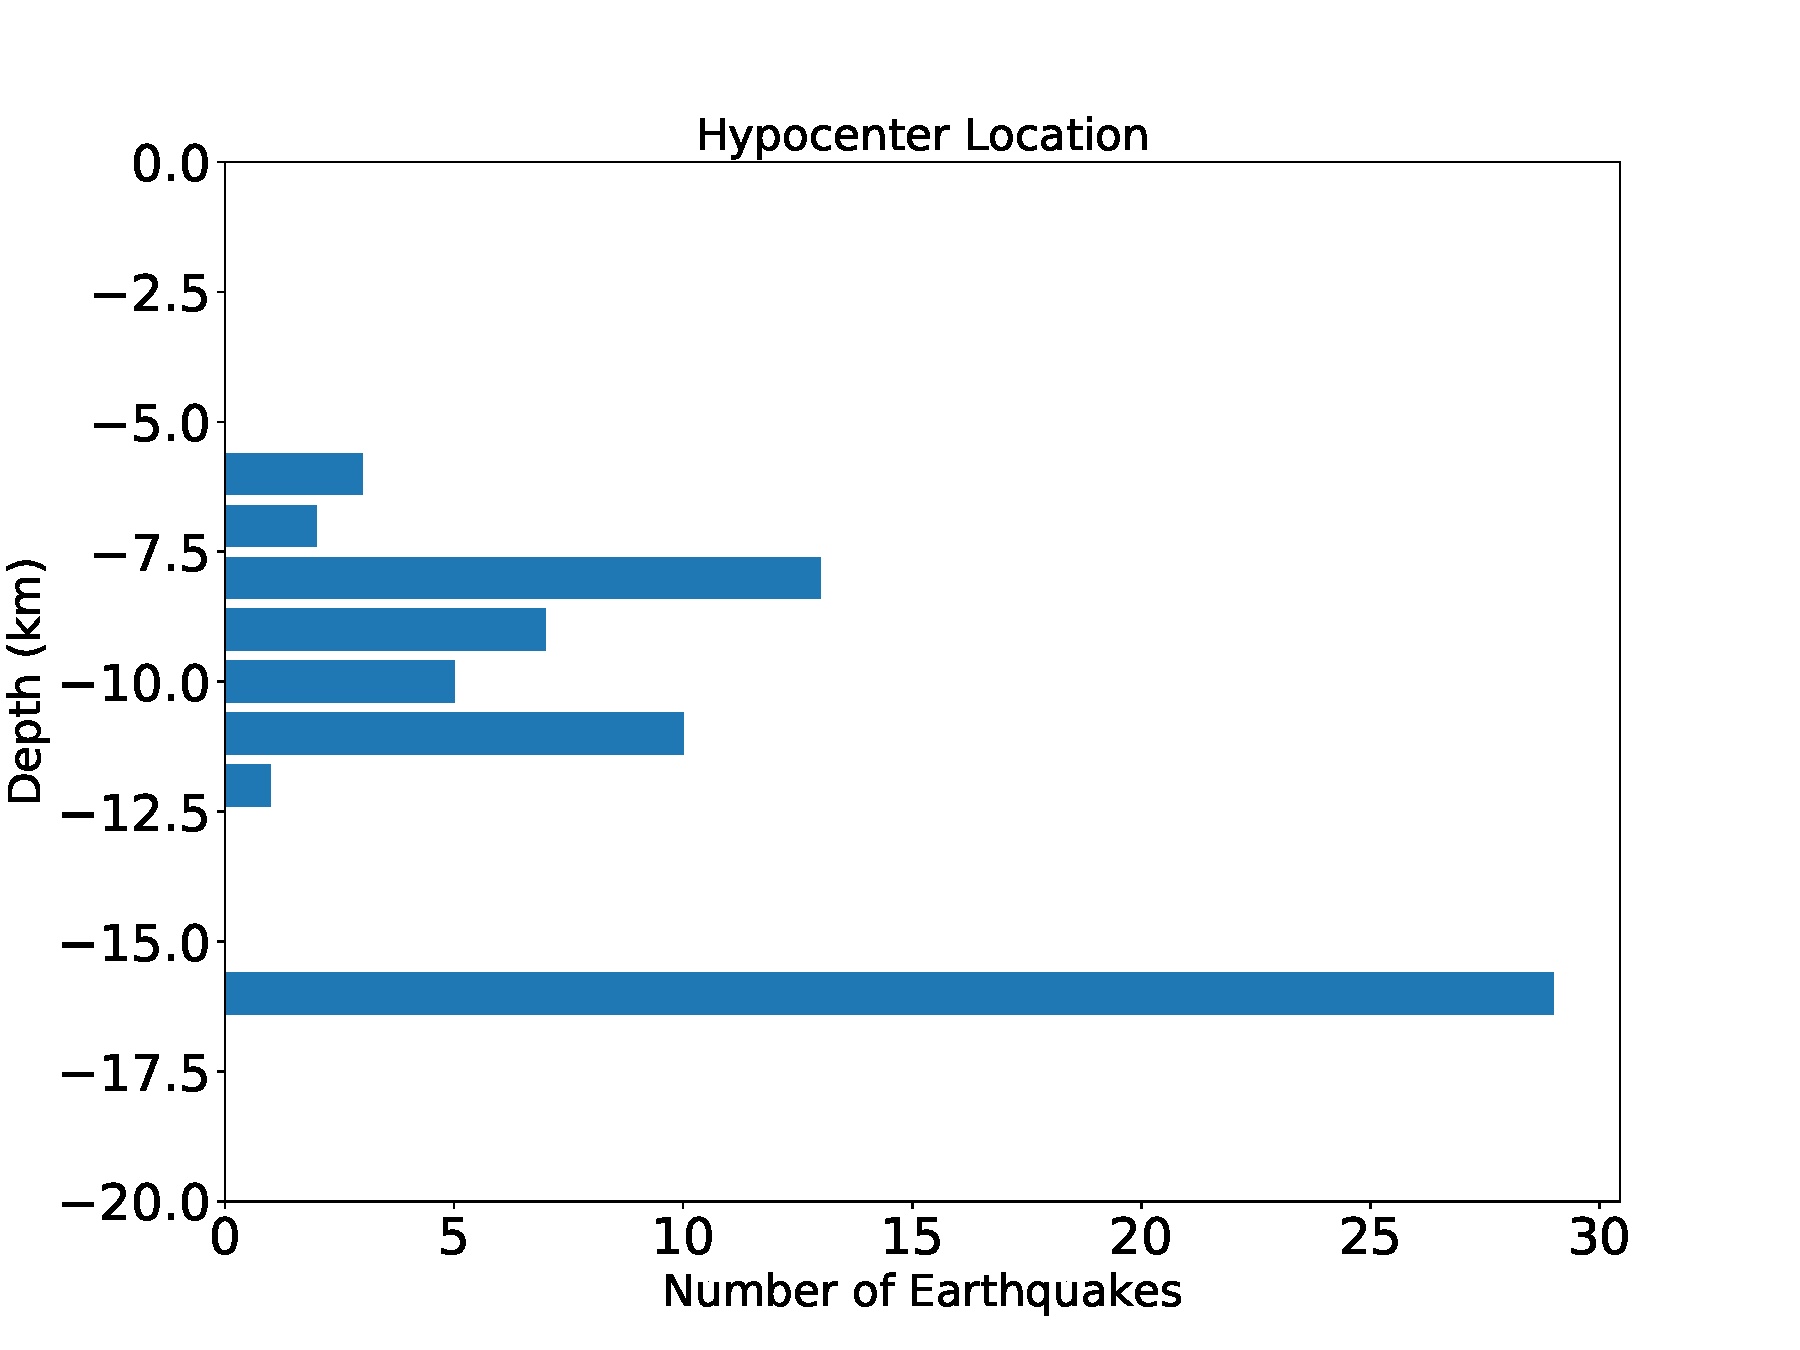
\includegraphics[width=\textwidth]{images/longfz.pdf} 
        \end{subfigure}%
        \begin{subfigure}[b]{0.5\textwidth}
            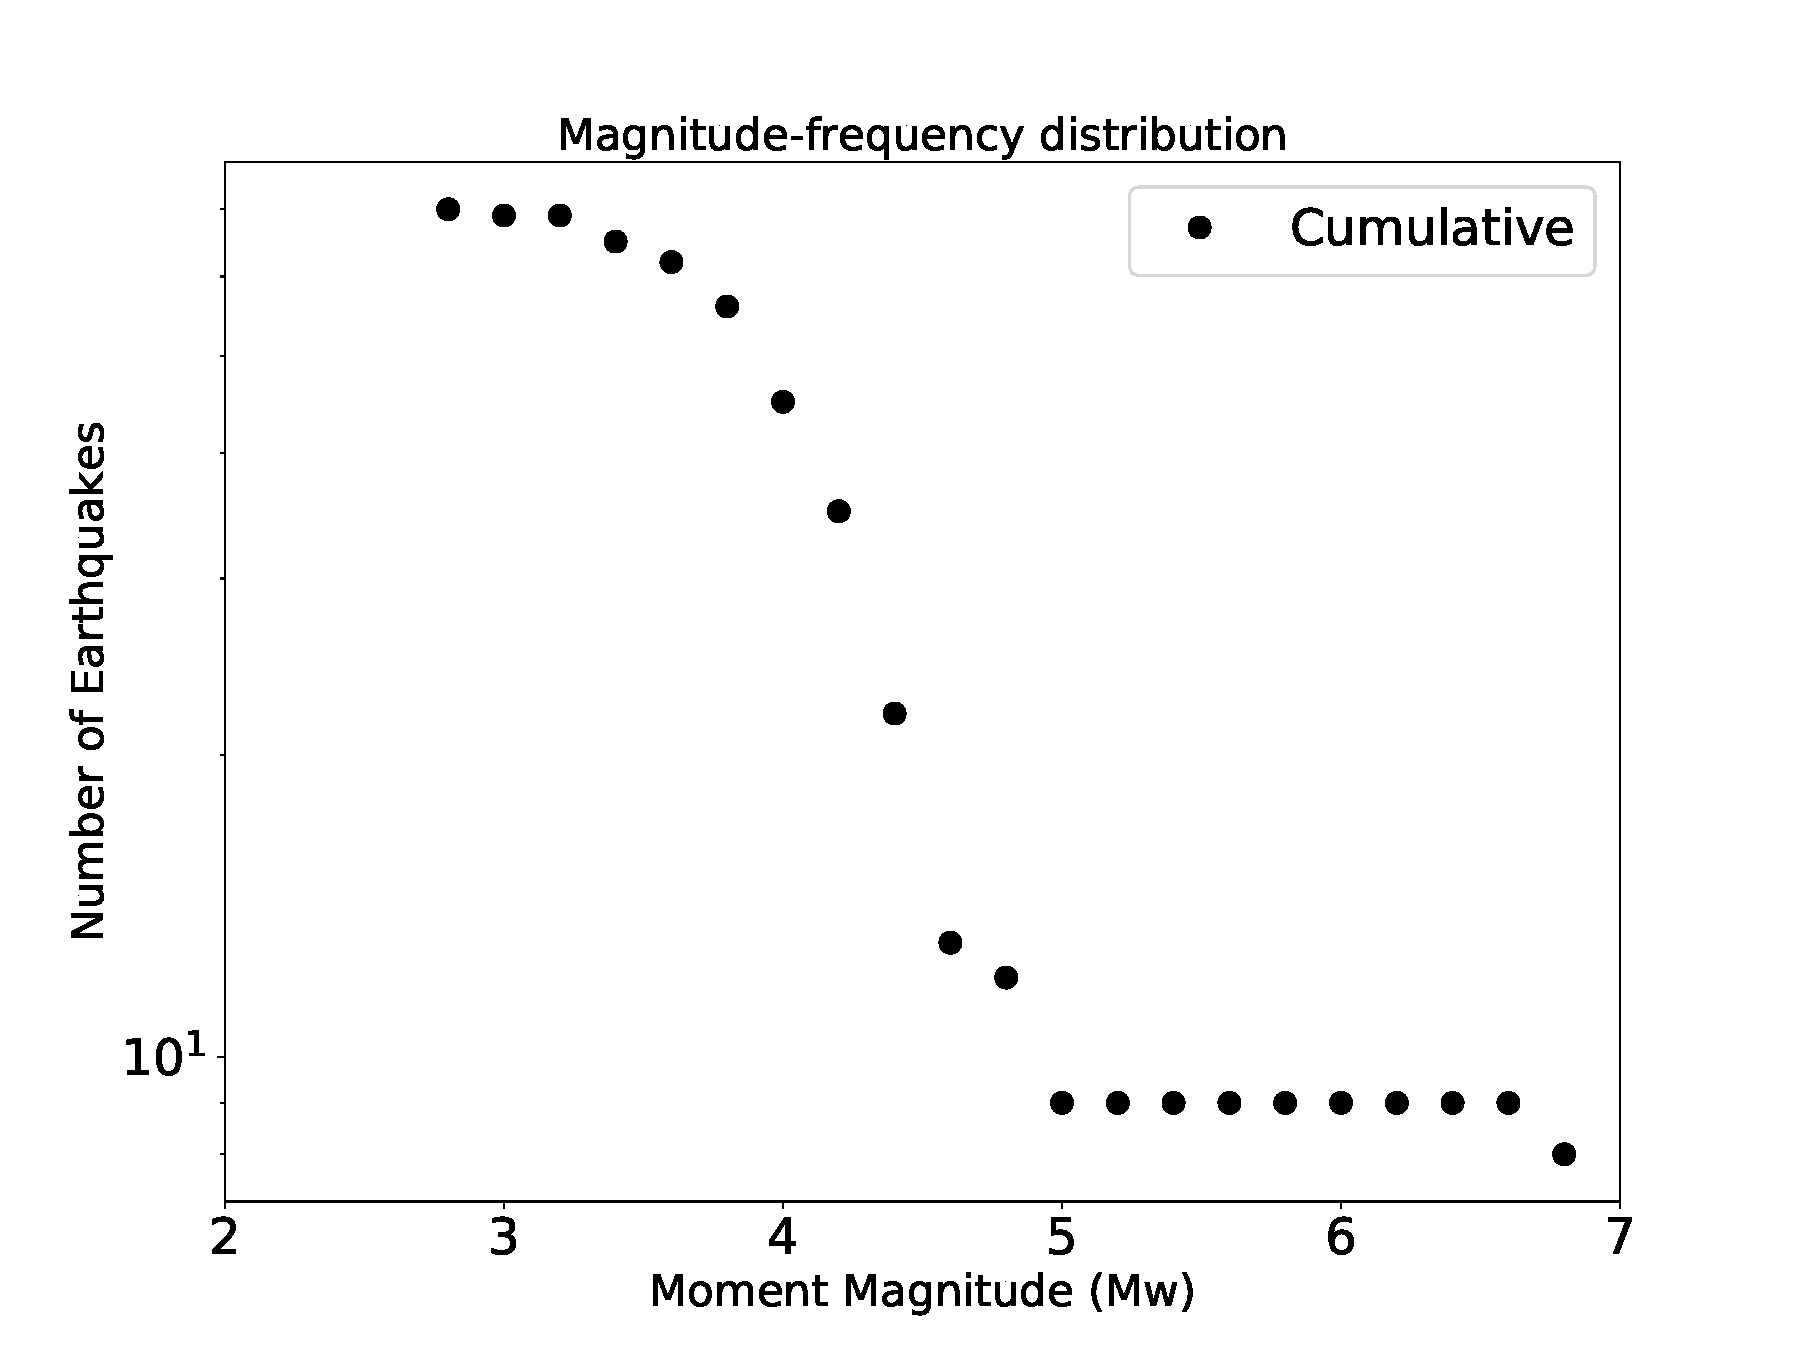
\includegraphics[width=\textwidth]{images/longfz_mfd.pdf}
        \end{subfigure}%
    \end{figure}
\end{frame}
\begin{frame}
    \frametitle{Simulated Results: Shallow Fault Zone: 8km deep }
    \begin{figure}
        \begin{subfigure}[b]{0.5\textwidth}
            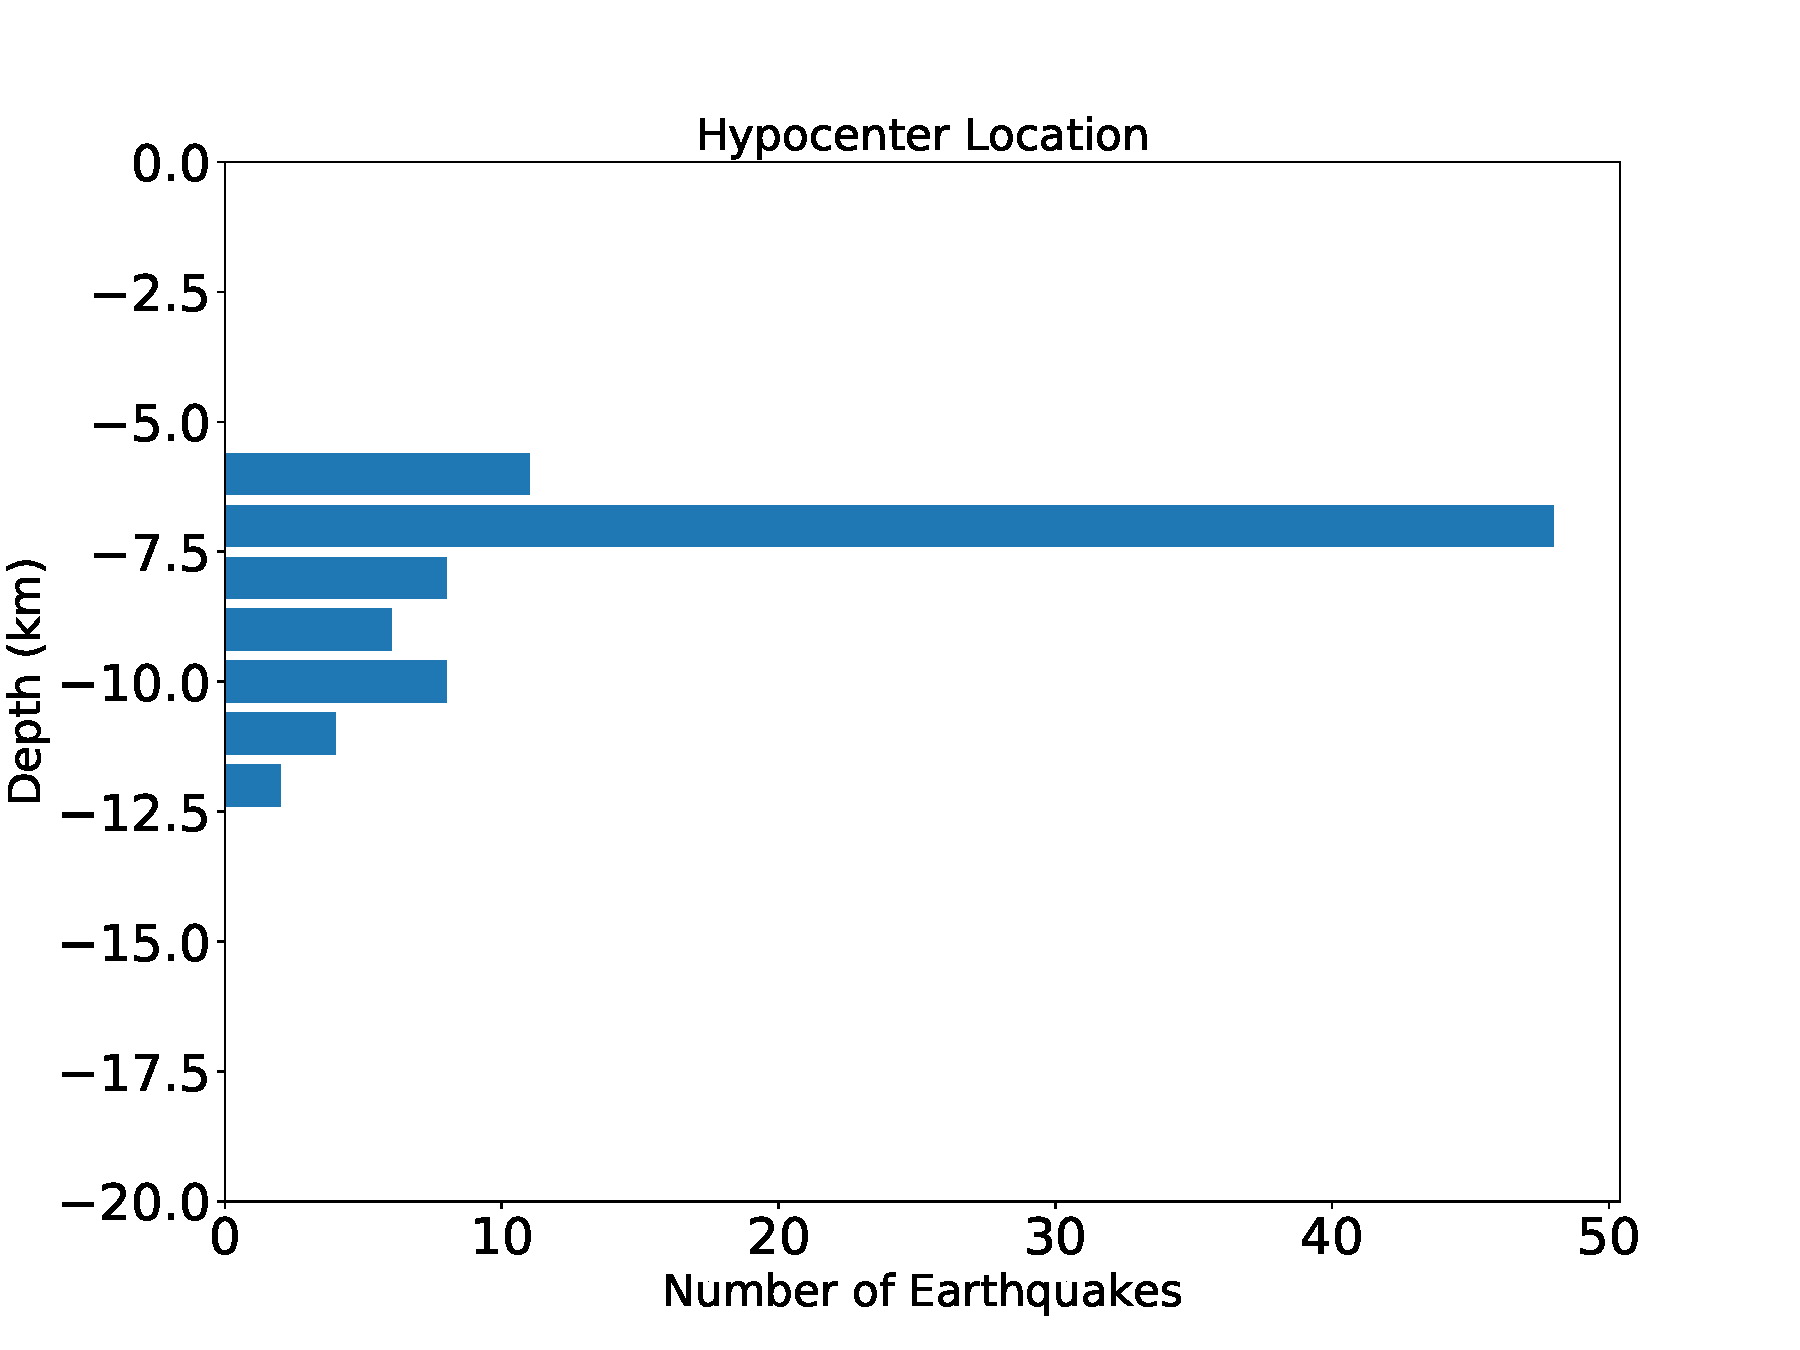
\includegraphics[width=\textwidth]{images/shallowfz.pdf} 
        \end{subfigure}%
        \begin{subfigure}[b]{0.5\textwidth}
            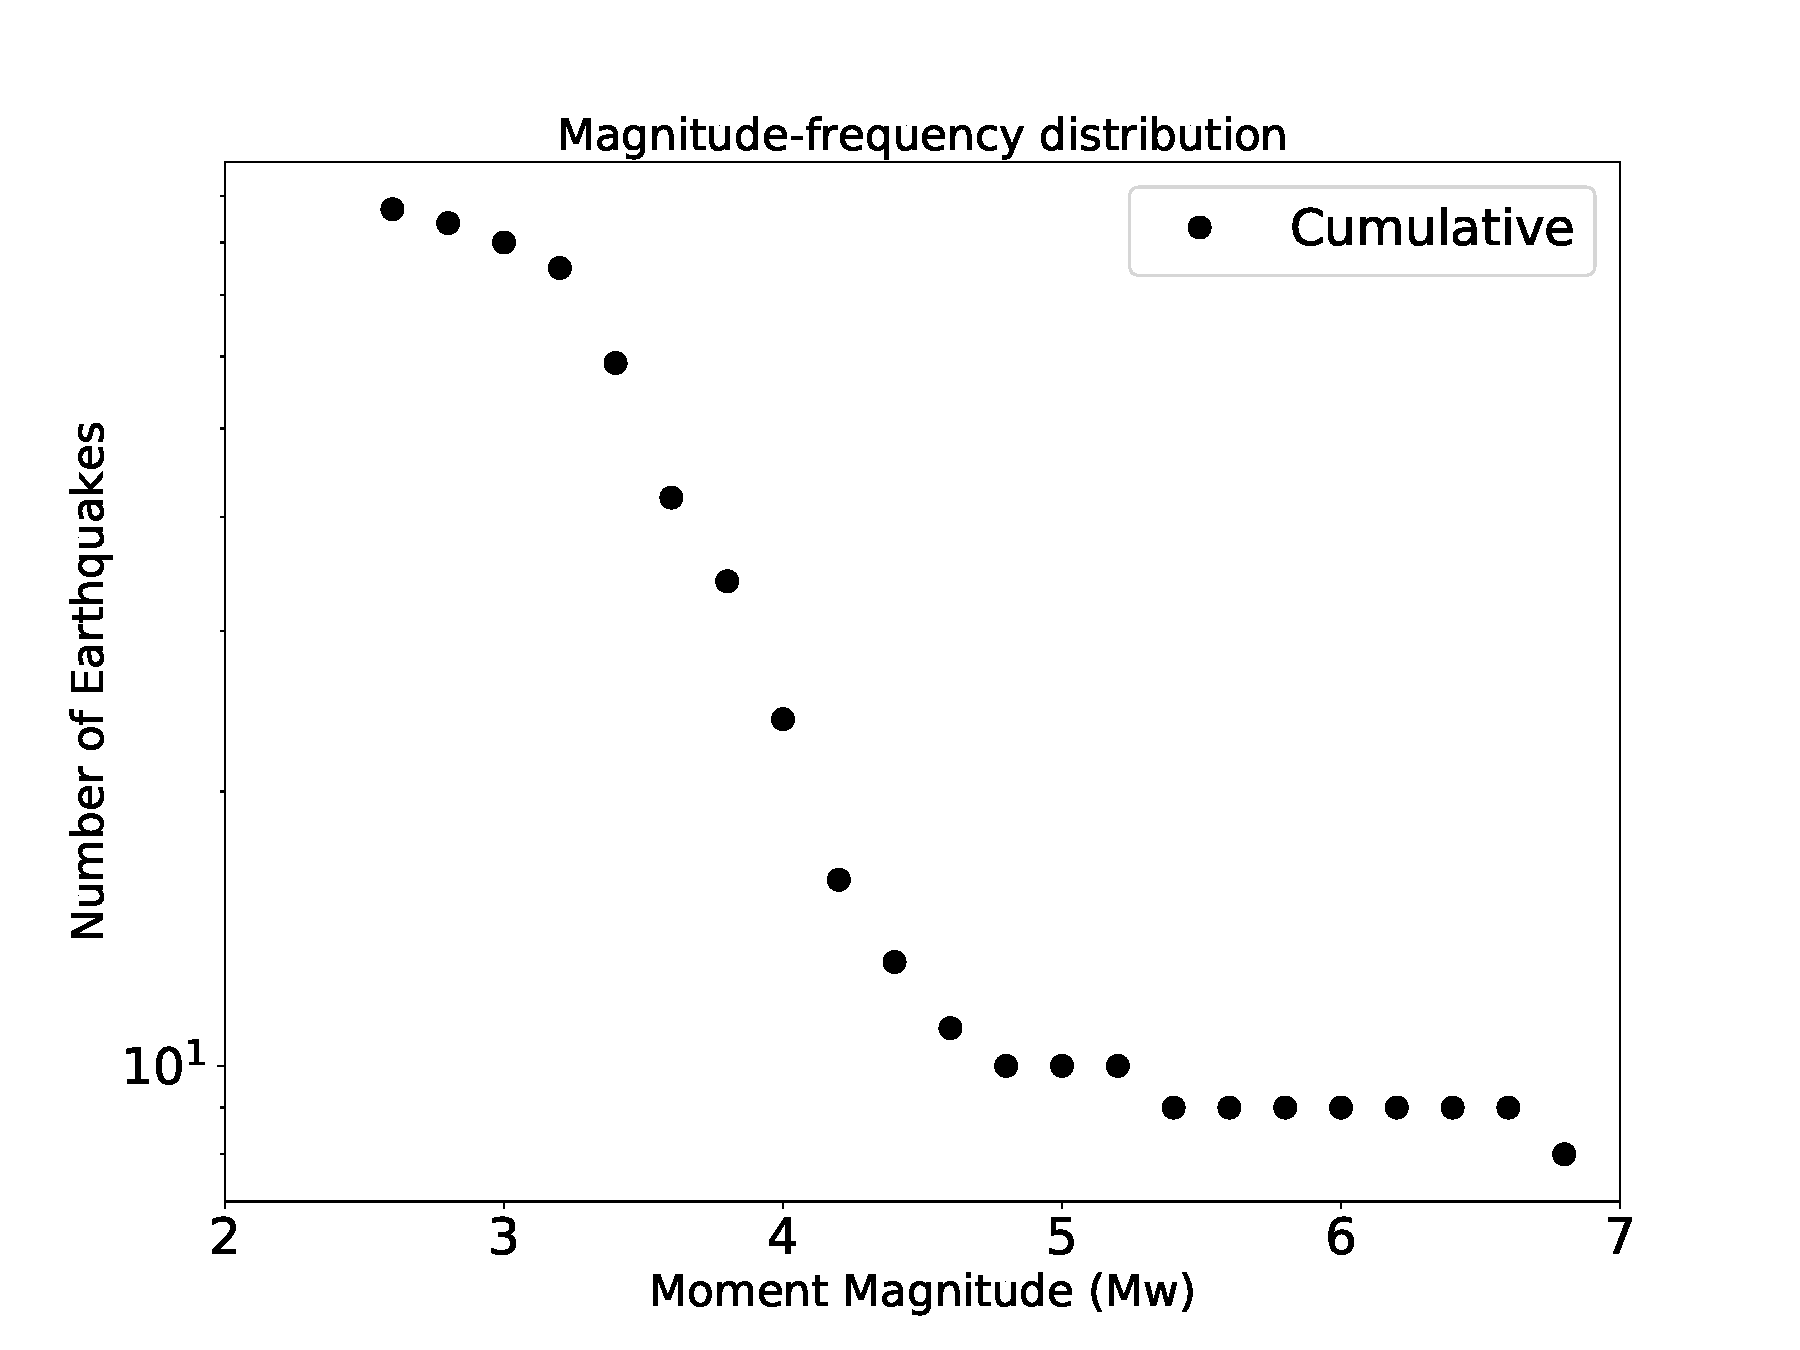
\includegraphics[width=\textwidth]{images/shallowfz_mfd.pdf}
        \end{subfigure}%
    \end{figure}
\end{frame}
\begin{frame}
    \frametitle{Simulated Results: Nested Fault Zone-Trapezoid Shaped}
    \begin{figure}
        \begin{subfigure}[b]{0.5\textwidth}
            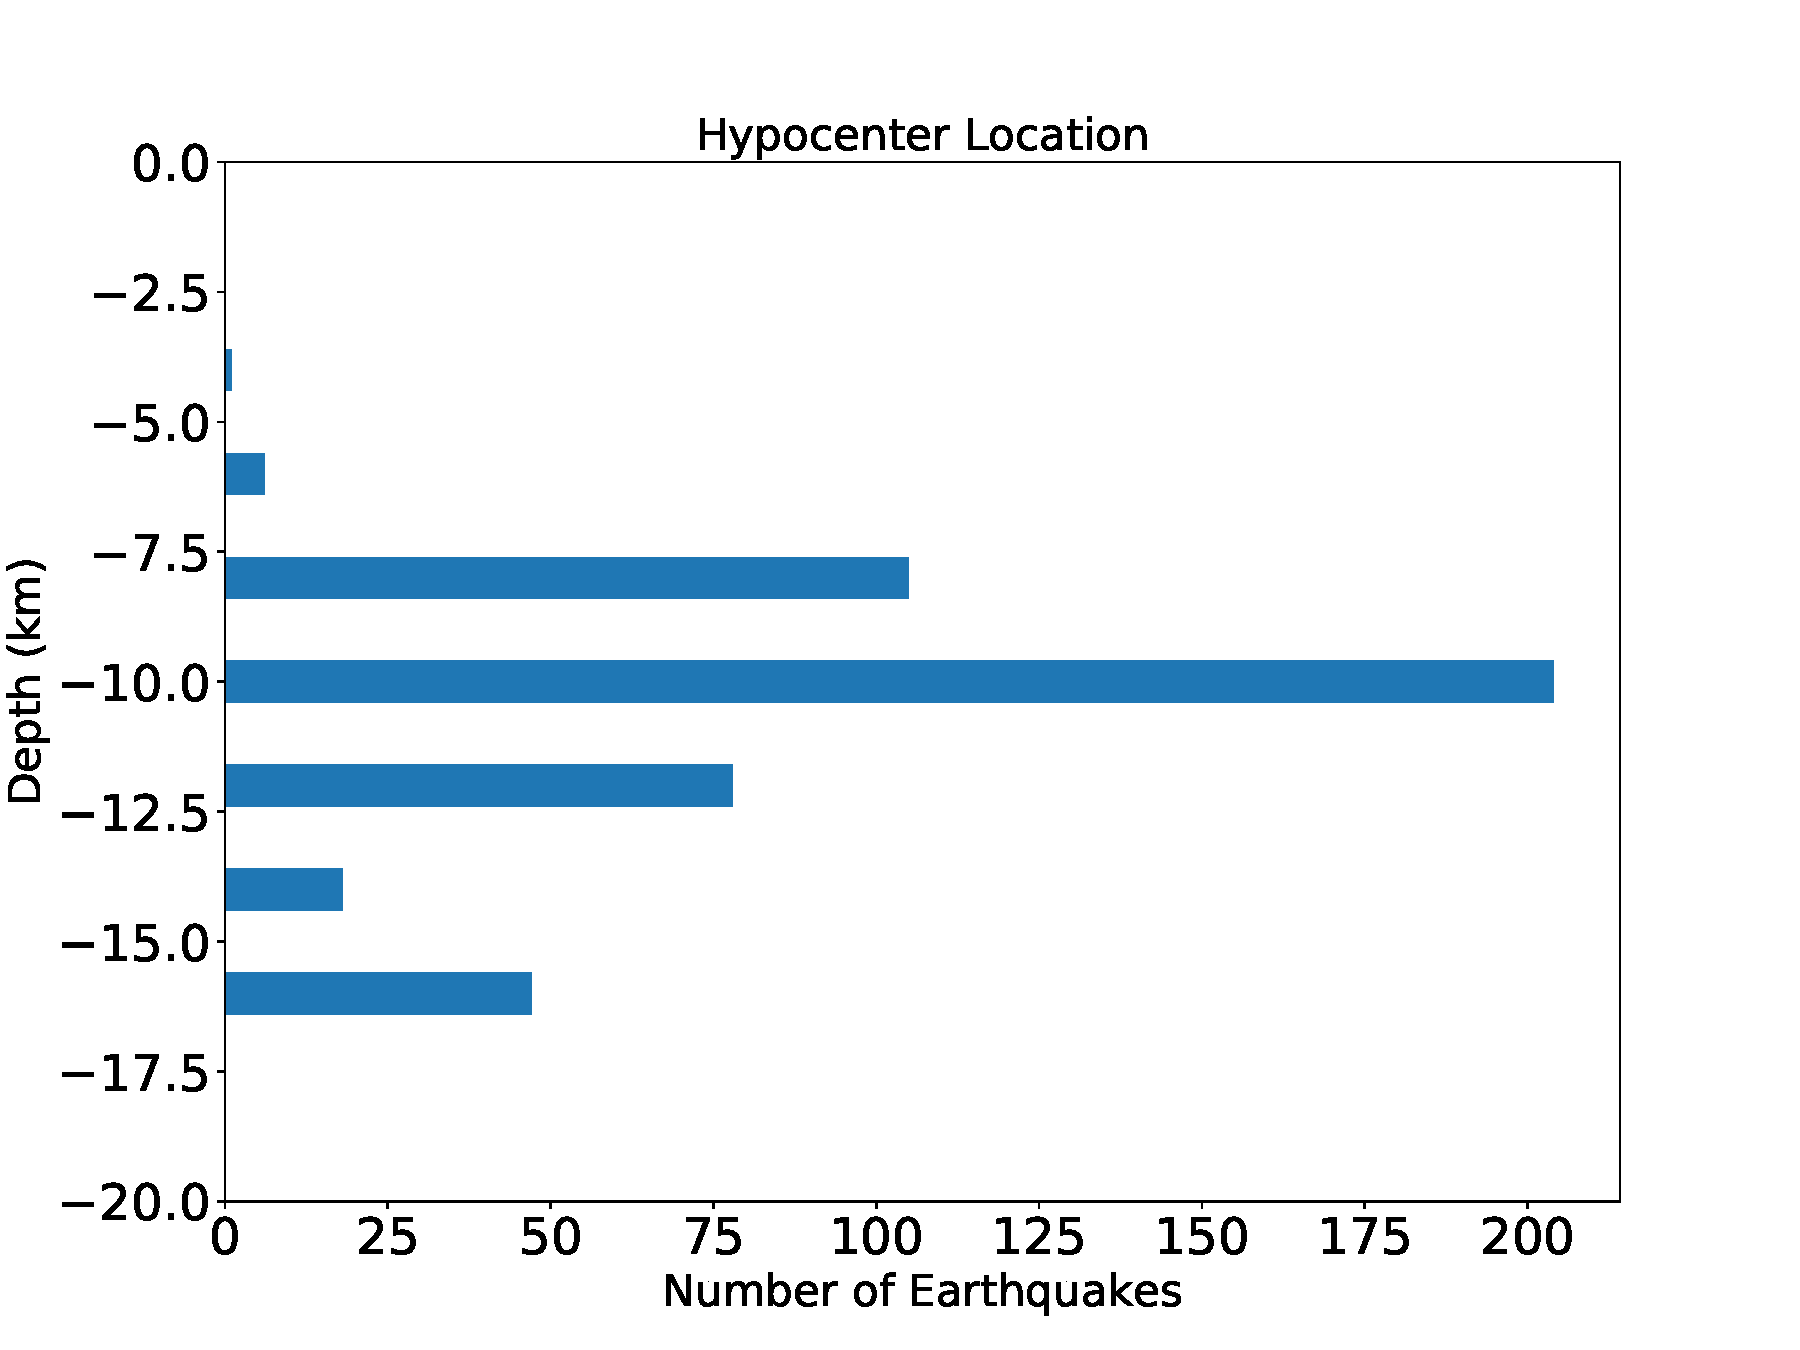
\includegraphics[width=\textwidth]{images/trap.pdf} 
        \end{subfigure}%
        \begin{subfigure}[b]{0.5\textwidth}
            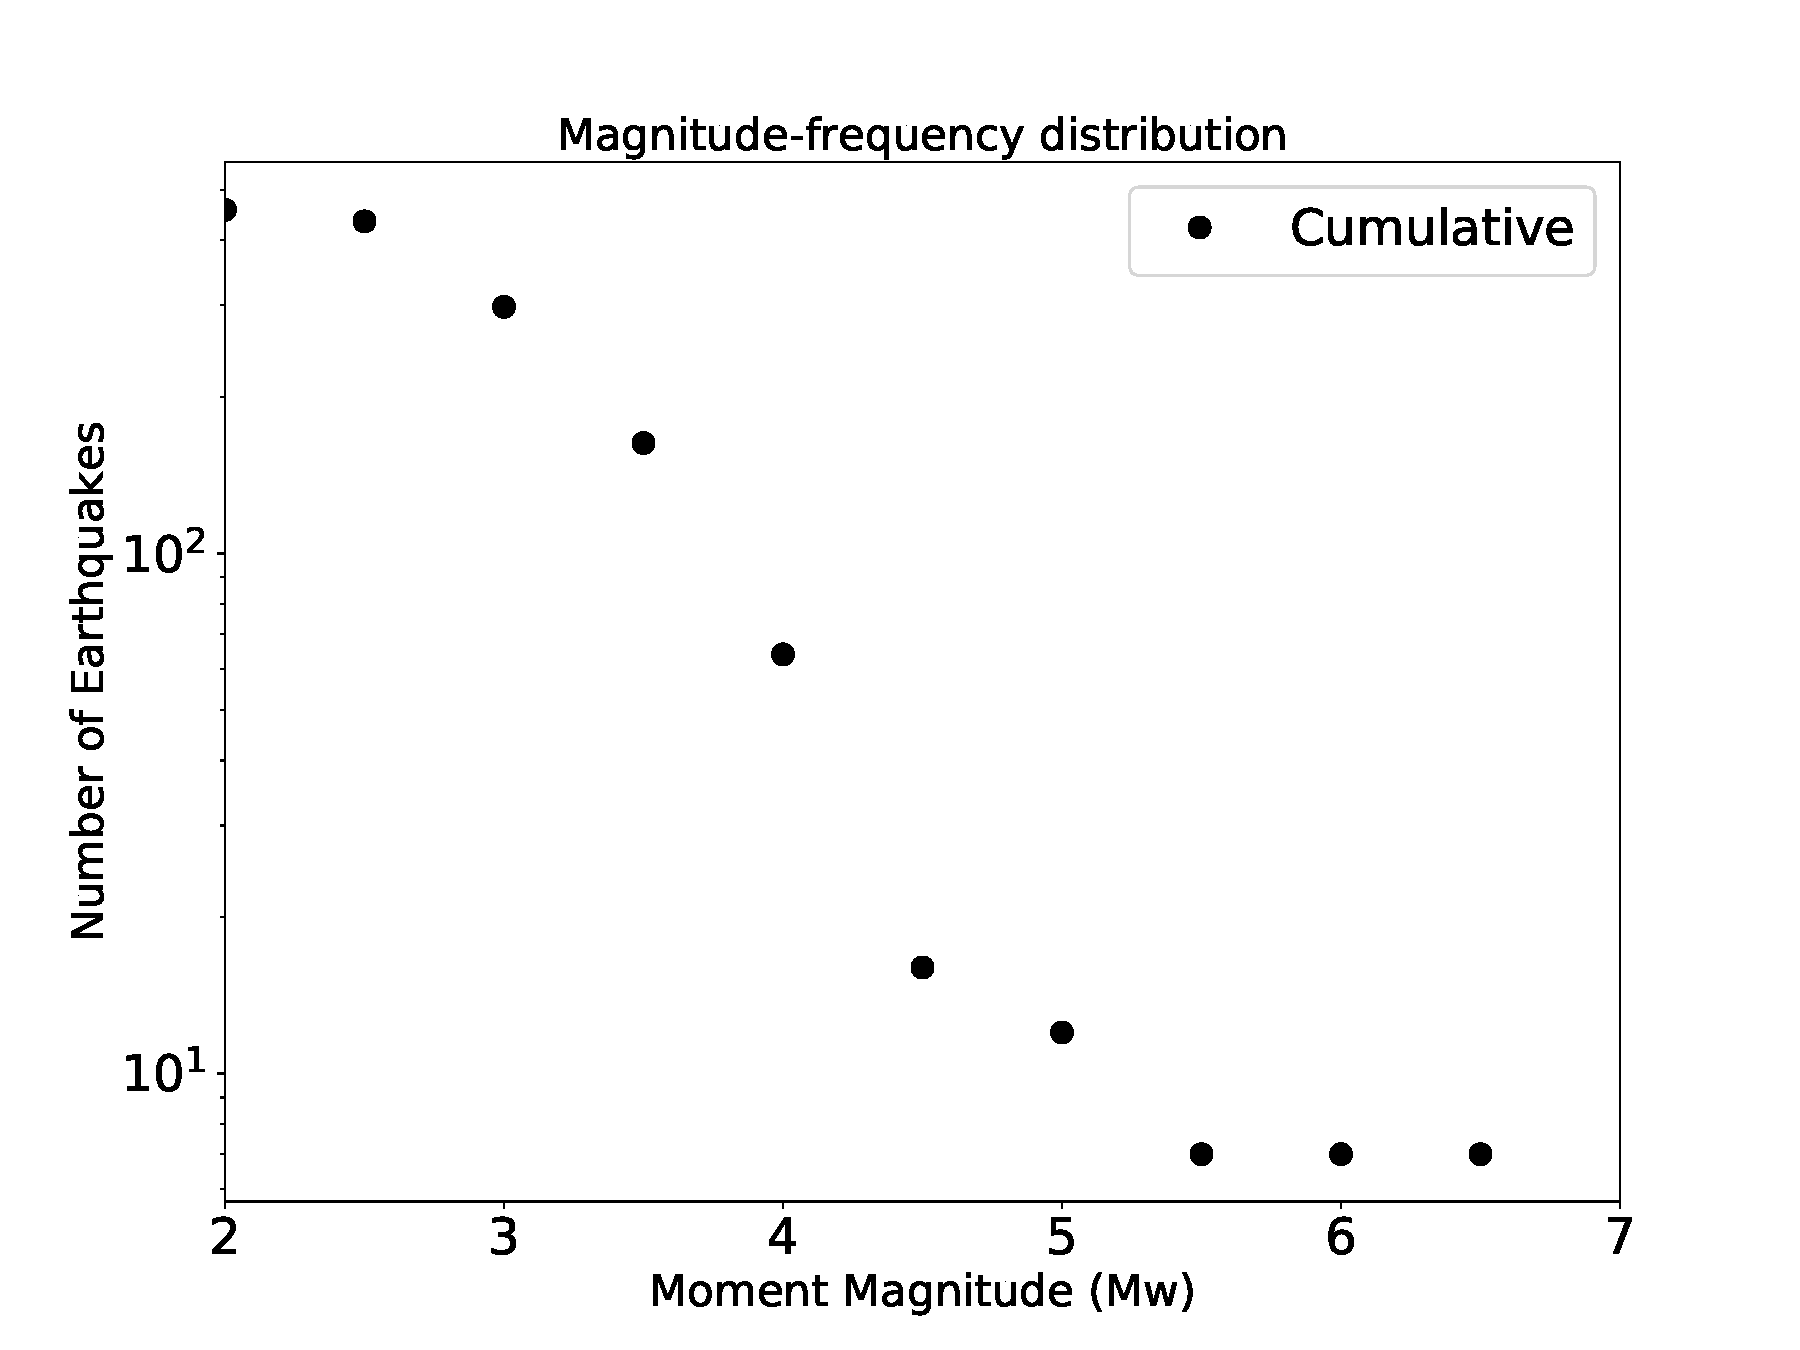
\includegraphics[width=\textwidth]{images/trap_mfd.pdf}
        \end{subfigure}%
    \end{figure}
\end{frame}

% Shear stress peaks
\begin{frame}
    \frametitle{Simulated Results: Shear Stress Distribution}
    \begin{figure}
        \begin{subfigure}[b]{0.5\textwidth}
            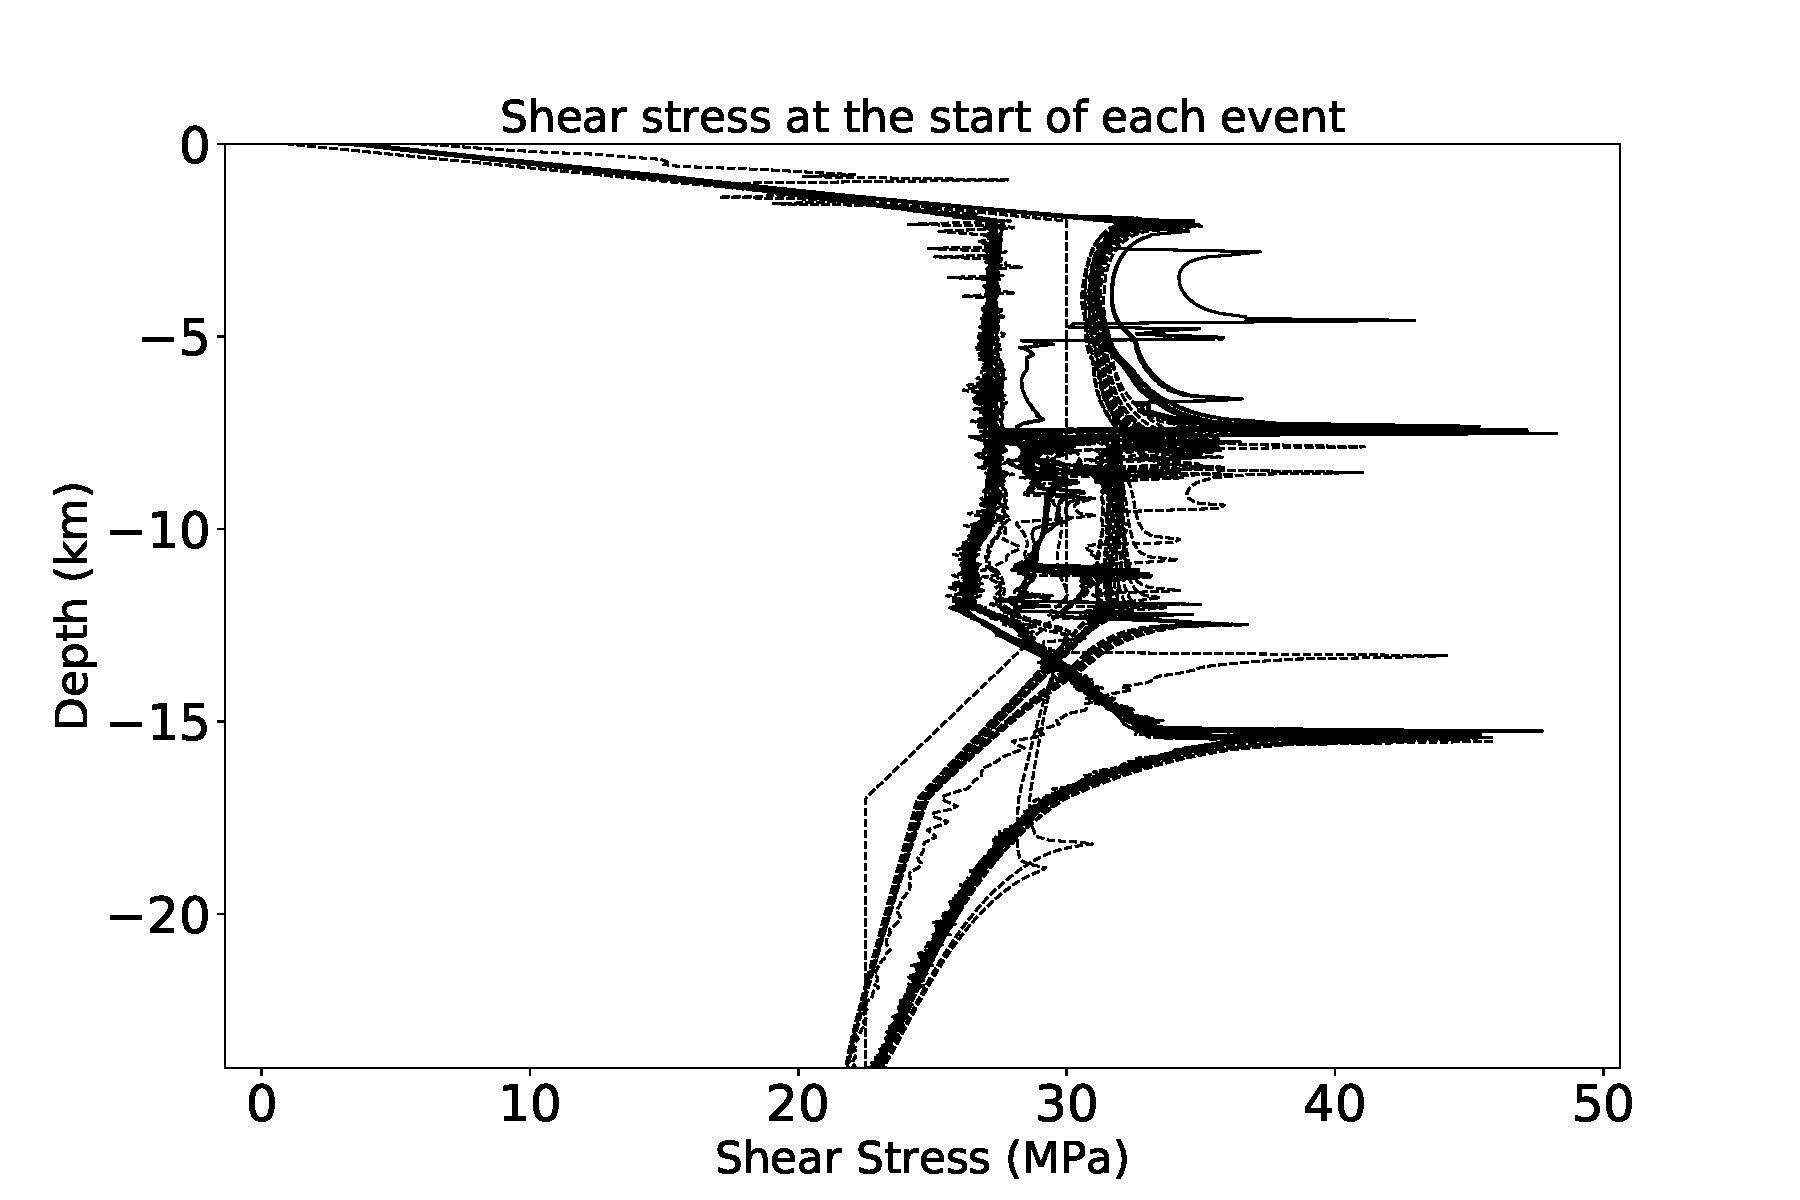
\includegraphics[width=\textwidth]{images/stress_event_deep.pdf} 
        \end{subfigure}%
        \begin{subfigure}[b]{0.5\textwidth}
            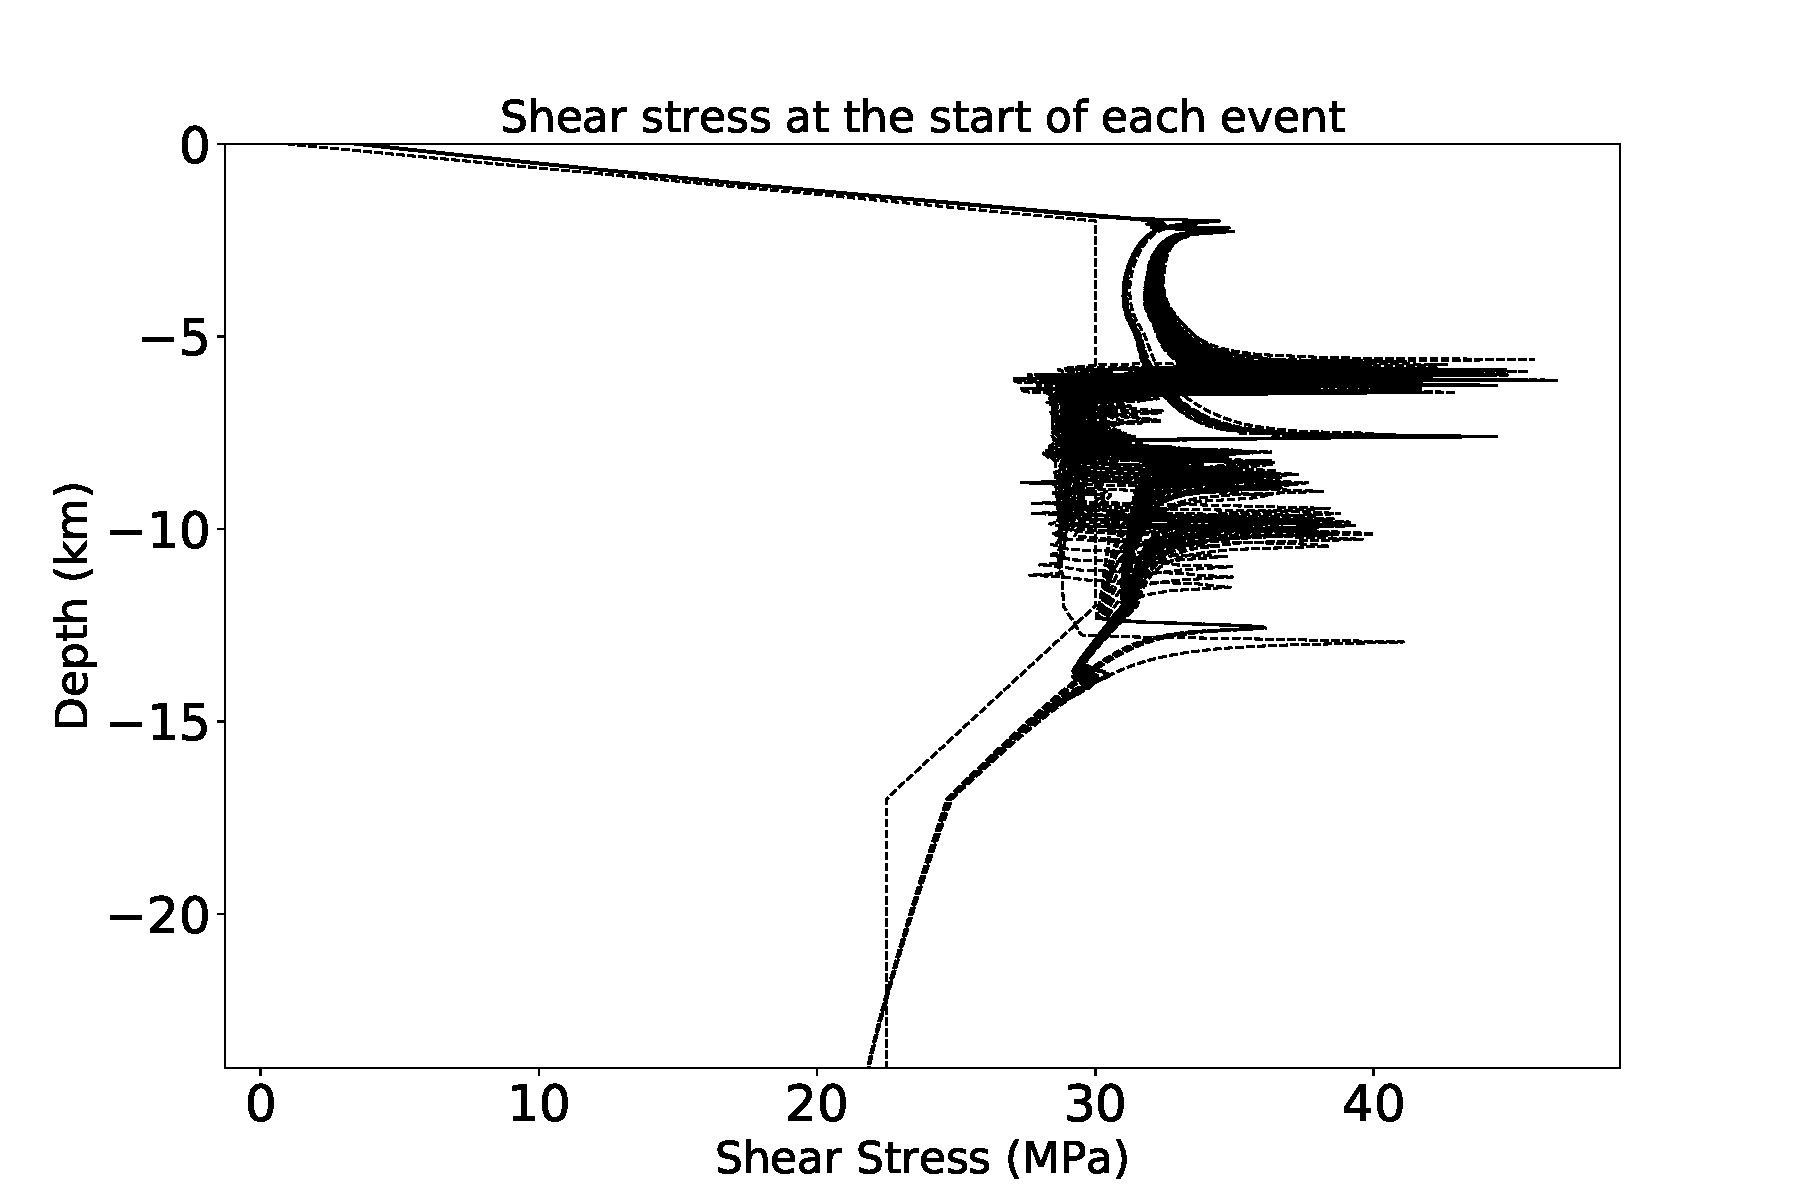
\includegraphics[width=\textwidth]{images/stress_event_shallow.pdf}
        \end{subfigure}%
    \end{figure}
    \setlength{\TPHorizModule}{\textwidth}
    \setlength{\TPVertModule}{\textwidth}
    \begin{textblock}{0.4} (0.17,0.2)
        Deep Fault Zone
    \end{textblock}
    \begin{textblock}{0.4} (0.67,0.2)
        Shallow Fault Zone
    \end{textblock}
\end{frame}


% CONCLUSIONS
\section{Conclusions}
\begin{frame}
    \frametitle{Conclusions}
    \begin{itemize}
        \item The presence of fault zone promotes stress heterogeneity.
        \item This stress heterogeneity gives rise to a power law distribution of earthquakes.
        \item The distribution is more similar to characteristic type earthquake distribution.
        \item Material heterogeneities are very common in the real faults and they can possibly explain some of the complexities in the earthquake behavior.
        \end{itemize}
\end{frame}

% FUTURE WORK
\section{Future Work}
\begin{frame}
\frametitle{Future Work}
    \item Damage Evolution: damage increment during seismic event and healing during interseismic periods
    \item Paleoseismic studies in Southern California: average recurrence of large earthquakes on multiple faults. How can we explain the variability in their recurrence? Are the large earthquakes on adjacent faults independent of each other?
    \item Geological outcrops can tell us about older damged zone architecture in great detail. How do the different geometries (flower structure vs hourglass structure) affect the evolution of slip and stress over multiple earthquake sequences?
    \item Write a code for Mode II rupture: dip-slip faults and along-strike variations in strike-slip faults.
\end{frame}

% ENDING SLIDE
\begin{frame}
    \Huge{\centerline{That's All Folks!!}}
\end{frame}
\end{document} 
%%%%%%%%%%%%%%%%
